\begin{table}
\begin{center}
\begin{tabular}{c|c|c|c}
\hline
Dataset & Subjects, Classes  & Train/Test & Neurovault collection 
\\ \hline
hcp~\cite{van2013wu}  & 787, 23 & 100/687  & collection 4337
\\
cam-can \cite{shafto2014cambridge}  & 605, 5 & 100/505  & collection 4342
\\
brainomics \cite{orfanos2017brainomics}  & 94, 19 & 50/44  &  collection 4341
\\
archi \cite{pinel2019functional}  & 78, 30 & 40/38  & collection 4339
\\
la5c \cite{poldrack2016phenome}  & 191, 24 & 100/91  & collection 4343
\\
pinel2012archi \cite{pinel2019functional} & 76, 10 & 40/36  & collection 1952
\\
pinel2009twins \cite{pinel2013genetic}  & 65, 12 & 35/30  & collection 1952
\\
pinel2007fast \cite{pinel2007fast} & 133, 10 & 70/63  & collection 1952
\\\hline\hline
\end{tabular}
\end{center}
\caption{\textbf{Datasets used in the experiments.} The table provides
  references to the datasets that were used for our experiments, with
  the number of subjects, the number of classes, the number of subjects in train
  and test set in each cross validation split and the collection number in Neurovault}
  \label{app:dataset:tab}
\end{table}

\begin{center}
  \begin{longtable}{ p{.11\textwidth} | p{.3\textwidth} |p{.5\textwidth}}
\hline
  Methods & Optimizer & Hyper-parameters \\
  \hline
LogReg & L-BFGS \newline ($20~000$ iterations) & inverse $L_2$ regularization
strength \newline in $\{0.0001, 0.001, 0.01, 0.1, 1 \}$ \\
  \hline
LDA  & Least-squares solver & Estimation of covariance \newline using Ledoit-Wolf's
                              method \\
  \hline
  RF &  - &  Default parameters in sklearn \\
  \hline
MLP  & Adam \newline ($20~000$ iterations, \newline momentum: $0.9$, \newline
batch size: $32$, \newline learning
       rate: $0.0001$) & $ReLU$ activation function, fully connected
                         architecture with two hidden layers both of size $1024$, L2
                         penalty coefficient: $10^{-5}$ \\
\hline \hline
\caption{\textbf{Optimizers and hyper-parameters of classifiers} For each classifier, we give the optimization method used as well as the value of hyper-parameters.}\label{app:classifiers:tab} 
\end{longtable}
 
\end{center}

\begin{table}
\begin{center}
\begin{tabular}{c|c|c|c}
\hline
Models & LDA  & LogR & MLP
\\ \hline
Original & P $\leq$ 0.01 & P $\leq$ 0.05 & P $\leq$ 0.0001 \\
 ICA & P $\leq$ 0.0001 & P $\leq$ 0.001 & P $\leq$ 0.001 \\
Covariance & P $\leq$ 0.05 & P $\leq$ 0.01 & P $\leq$ 0.05 \\
ICA + Covariance & P $\leq$ 0.0001 & P $\leq$ 0.0001 & P $\leq$ 0.01 \\
GANs & P $\leq$ 0.001 & P $\leq$ 0.001 & P $\leq$ 0.0001 \\
CGANs & P $\leq$ 0.001 & P $\leq$ 0.01 & P $\leq$ 0.0001 \\
\hline\hline
\end{tabular}
\end{center}
\caption{\textbf{Statistical significance of the differences between Conditional ICA and other augmentation methods} P-values obtained after a t-test for paired samples is performed on the data used to produce Table~\ref{tab3}}\label{app:significance}
\end{table}

\begin{table}
\begin{center}
\begin{tabular}{c|c|}
\hline
Models & RF \\
\hline
Original & 0.782 \\
ICA & 0.778 \\
COV. & 0.780 \\
ICA + COV. & 0.780 \\
GANs & 0.780 \\
CGANs & 0,779 \\
Cond. ICA & 0.783 \\
\hline\hline
\end{tabular}
\end{center}
\caption{\textbf{Accuracy of Random Forrest} Mean accuracy obtained on data used to produce Table~\ref{tab3} with a Random Forest classifier depending on the chosen augmentation method}\label{app:randomforrest}
\end{table}

\begin{table}
\begin{center}
\begin{tabular}{|c|c|}
\hline
Methods & Running-time (secs)
\\ \hline
GANs  & 12948.2 ($\approx$ 3,60 hr)
\\
CGANs  & 11015.1 ($\approx$ 3,05 hr)
\\
\textbf{Conditional ICA}  & 62 s 
\\
\hline
\end{tabular}
\end{center}
\caption{\textbf{Running time.} We display the running time of three methods used
  to generate synthetic data. Conditional ICA is several orders of magnitude faster than
  GANs or CGANs. In practice the computational over-head induced by Conditional ICA is negligible.}\label{app:runningtime:tab}
\end{table}



\begin{figure}
  \centerline{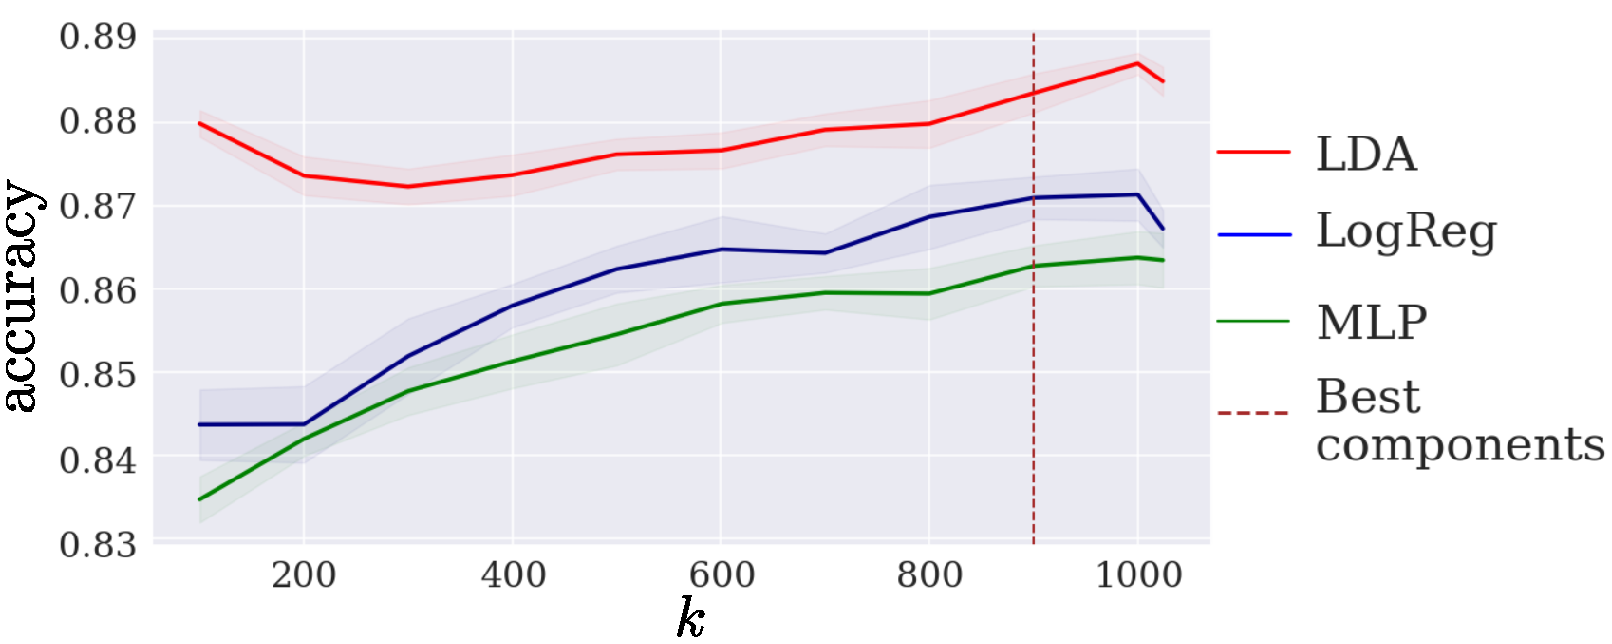
\includegraphics[width=0.8\textwidth]{figures/condica/sensitivity.pdf}}
  \caption{\textbf{Accuracy of augmented discriminative models when
      varying $k$.} We use 100 train subjects from the HCP task dataset to train Conditional ICA with $k$ components and generate $200$ fake subjects.
    Classifiers are trained on the train and fake subjects and tested on the
    left-out 687 subjects. We repeat the procedure
    for various values of $k$ using 5 random splits per value and
    report the mean accuracy across splits as a function of $k$.
    The dotted line represents the number of components that has been
    used in our experiments ($k=900$).
  }
  \label{app:sensitivity:fig}
\end{figure}



\begin{figure}
  \centerline{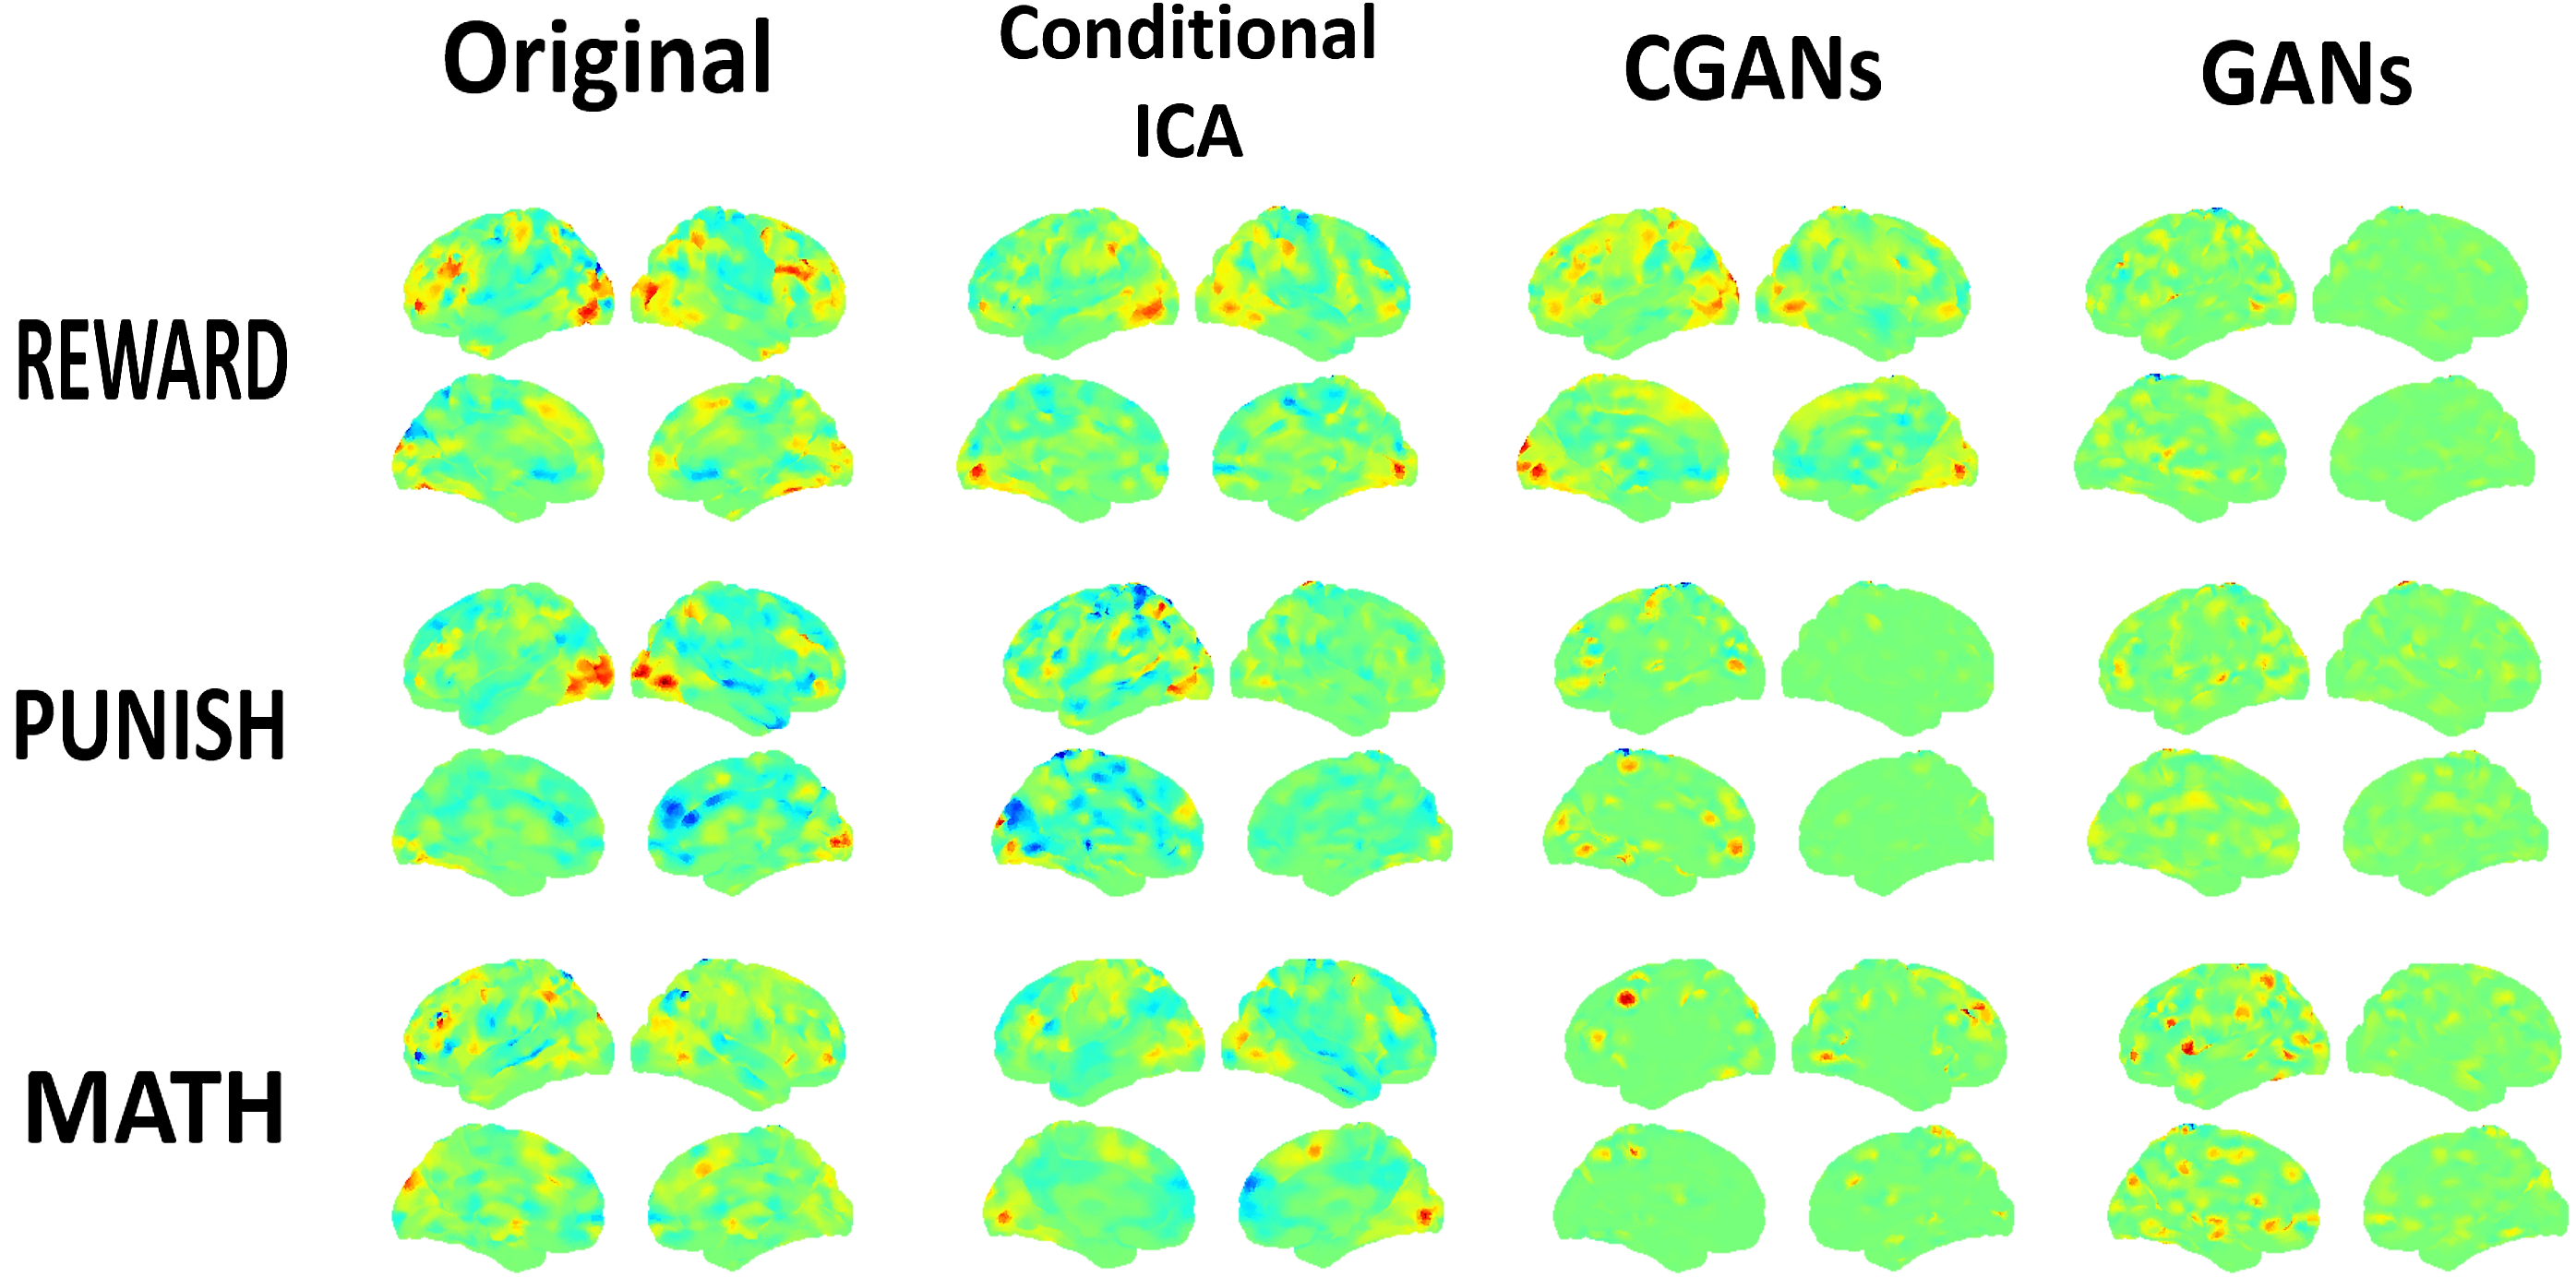
\includegraphics[width=0.8\linewidth]{figures/condica/fake_real_viz_v3_redim_improved.png}}
  \caption{\textbf{Data generation visualization.} Visualization of real
    (Original) and synthetic brain maps from three generation methods:
    Conditional ICA, CGANs and GANS. Three cognitive tasks are shown (reward, punish and math).
  }
  \label{app:visualization:fig}
\end{figure}
